\documentclass[12pt]{article}
\usepackage[T1]{fontenc}
\usepackage{algorithm2e}
\usepackage{dot2texi}

\usepackage{tikz}
\usepackage{listings}
\usepackage{float}
\usetikzlibrary{shapes,arrows}
\usepackage{bchart}

\makeatletter
%%%%%%%%%%%%%%%%%%%%%%%%%%%%%% Textclass specific LaTeX commands.
\newenvironment{lyxlist}[1]
{\begin{list}{}
{\settowidth{\labelwidth}{#1}
 \setlength{\leftmargin}{\labelwidth}
 \addtolength{\leftmargin}{\labelsep}
 \renewcommand{\makelabel}[1]{##1\hfil}}}
{\end{list}}

%%%%%%%%%%%%%%%%%%%%%%%%%%%%%% User specified LaTeX commands.
\usepackage{sbc-template}

\usepackage[brazil]{babel}
\usepackage[utf8]{inputenc}

\sloppy

\title{Arizona Jones}

\author{Pedro Vanzella\inst{1}}

\address{Faculdade de Informática -- Pontifícia Universidade Católica do Rio
Grande do Sul (PUCRS) \\ Av. Ipiranga, 6681 - Porto Alegre / RS / Brasil
    \email pedro@pedrovanzella.com}

\makeatother

\usepackage{babel}
\usepackage{listings}
\lstset {
    mathescape,
    frame=none
}
\renewcommand{\lstlistingname}{Listagem}

\begin{document}

\maketitle
\begin{resumo}
  Uma solu\c{c}ão para o problema do Arizona Jones no Templo de Tel Dor é proposta. Um grafo é montado com os dados de entrada, e o maior caminho no mesmo representa a solução do problema.
\end{resumo}


\section{Introdução}\label{sec:intro}

O problema a ser resolvido consiste em encontrar, dentro de um conjunto de números, a maior seqüência crescente de números que, em base 6, têm somente um dígito de diferen\c{c}a entre um e outro. 

Por exemplo, no conjunto $782$ $229$ $446$ $527$ $874$ $19$ $829$ $70$ $830$ $992$ $430$ $649$, a maior seqüência é $649$ $829$ $830$.

Para isto, os números são organizados em um grafo e o maior caminho é encontrado. Como veremos na se\c{c}ão~\ref{sec:algoritmos:achar-maior-caminho}, isto é uma opera\c{c}ão que roda em tempo linear, gra\c{c}as a algumas propriedades interessantes deste grafo.

\section{Estruturas de Dados}\label{sec:estruturas}
Vamos representar o conjunto de números como um grafo. Isto nos permitirá ligar os nodos que formam seqüências válidas e encontrar a maior seqüência, procurando pelo maior caminho.

Para representar internamente o grafo, utilizamos três dicionários: um dicionário para nodos, um para arestas e um para o peso dos nodos. Este último será explicado em detalhe nas se\c{c}ões~\ref{sec:algoritmos:achar-maior-caminho} e~\ref{sec:algoritmos:calcular-tamanho-caminhos}.

O dicionário de nodos tem uma propriedade interessante: seu índice é o número em base 10, como foi lido do arquivo; seu conteúdo é a representa\c{c}ão em base 6 do mesmo número, como um array de dígitos, para facilitar a compara\c{c}ão. Esta representa\c{c}ão é guardada no array de modo a evitar o recálculo da conversão de base, trocando processamento por memória.

Este grafo é dirigido e acíclico. Isto fica óbvio quando pensamos nos parâmetros do problema: se, para criar uma aresta, precisamos ligar um nodo a alguém maior que ele, não podemos ter ciclos (i.e. A não pode ser maior que B ao mesmo tempo que B é maior que A). Como veremos na se\c{c}ão~\ref{sec:algoritmos:achar-maior-caminho}, isto é muito bom para nós.

% TODO: EXPLICAR ISTO!
%O grafo é dirigido e acíclico, então o algoritmo de encontrar o maior caminho é O(n): https://en.wikipedia.org/wiki/Longest_path_problem

Podemos ver na Figura~\ref{fig:testeprof} um grafo gerado de acordo com o exemplo dado na se\c{c}ão~\ref{sec:intro}

\begin{figure}[H]
  \noindent %
  \begin{minipage}[t]{0.3\columnwidth}%
    \begin{figure}
        \begin{lstlisting}
        782
        229
        446
        527
        874
        19
        829
        70
        830
        992
        430
        649
        \end{lstlisting}
        \caption{Arquivo de Entrada}
        \label{fig:testeprof:entrada}
      \end{figure}
  \end{minipage}
  \begin{minipage}[t][1\totalheight][b]{0.65\textwidth}%
    \begin{figure}
        \begin{dot2tex}[neato,options=-tmath]
            \documentclass{article}
\usepackage[x11names, rgb]{xcolor}
\usepackage[utf8]{inputenc}
\usepackage{tikz}
\usetikzlibrary{snakes,arrows,shapes}
\usepackage{amsmath}
%
%

%

%

\begin{document}
\pagestyle{empty}
%
%
%

\enlargethispage{100cm}
% Start of code
% \begin{tikzpicture}[anchor=mid,>=latex',line join=bevel,]
\begin{tikzpicture}[>=latex',line join=bevel,]
  \pgfsetlinewidth{1bp}
%%
\pgfsetcolor{black}
  % Edge: 829 -- 830
  \draw [] (459.0bp,71.697bp) .. controls (459.0bp,60.846bp) and (459.0bp,46.917bp)  .. (459.0bp,36.104bp);
  % Edge: 649 -- 829
  \draw [] (459.0bp,143.7bp) .. controls (459.0bp,132.85bp) and (459.0bp,118.92bp)  .. (459.0bp,108.1bp);
  % Node: 830
\begin{scope}
  \definecolor{strokecol}{rgb}{0.0,0.0,0.0};
  \pgfsetstrokecolor{strokecol}
  \draw (459.0bp,18.0bp) ellipse (27.0bp and 18.0bp);
  \draw (459.0bp,18.0bp) node {830};
\end{scope}
  % Node: 782
\begin{scope}
  \definecolor{strokecol}{rgb}{0.0,0.0,0.0};
  \pgfsetstrokecolor{strokecol}
  \draw (27.0bp,162.0bp) ellipse (27.0bp and 18.0bp);
  \draw (27.0bp,162.0bp) node {782};
\end{scope}
  % Node: 992
\begin{scope}
  \definecolor{strokecol}{rgb}{0.0,0.0,0.0};
  \pgfsetstrokecolor{strokecol}
  \draw (603.0bp,162.0bp) ellipse (27.0bp and 18.0bp);
  \draw (603.0bp,162.0bp) node {992};
\end{scope}
  % Node: 19
\begin{scope}
  \definecolor{strokecol}{rgb}{0.0,0.0,0.0};
  \pgfsetstrokecolor{strokecol}
  \draw (387.0bp,162.0bp) ellipse (27.0bp and 18.0bp);
  \draw (387.0bp,162.0bp) node {19};
\end{scope}
  % Node: 874
\begin{scope}
  \definecolor{strokecol}{rgb}{0.0,0.0,0.0};
  \pgfsetstrokecolor{strokecol}
  \draw (315.0bp,162.0bp) ellipse (27.0bp and 18.0bp);
  \draw (315.0bp,162.0bp) node {874};
\end{scope}
  % Node: 446
\begin{scope}
  \definecolor{strokecol}{rgb}{0.0,0.0,0.0};
  \pgfsetstrokecolor{strokecol}
  \draw (171.0bp,162.0bp) ellipse (27.0bp and 18.0bp);
  \draw (171.0bp,162.0bp) node {446};
\end{scope}
  % Node: 527
\begin{scope}
  \definecolor{strokecol}{rgb}{0.0,0.0,0.0};
  \pgfsetstrokecolor{strokecol}
  \draw (243.0bp,162.0bp) ellipse (27.0bp and 18.0bp);
  \draw (243.0bp,162.0bp) node {527};
\end{scope}
  % Node: 829
\begin{scope}
  \definecolor{strokecol}{rgb}{0.0,0.0,0.0};
  \pgfsetstrokecolor{strokecol}
  \draw (459.0bp,90.0bp) ellipse (27.0bp and 18.0bp);
  \draw (459.0bp,90.0bp) node {829};
\end{scope}
  % Node: 229
\begin{scope}
  \definecolor{strokecol}{rgb}{0.0,0.0,0.0};
  \pgfsetstrokecolor{strokecol}
  \draw (99.0bp,162.0bp) ellipse (27.0bp and 18.0bp);
  \draw (99.0bp,162.0bp) node {229};
\end{scope}
  % Node: 70
\begin{scope}
  \definecolor{strokecol}{rgb}{0.0,0.0,0.0};
  \pgfsetstrokecolor{strokecol}
  \draw (531.0bp,162.0bp) ellipse (27.0bp and 18.0bp);
  \draw (531.0bp,162.0bp) node {70};
\end{scope}
  % Node: 649
\begin{scope}
  \definecolor{strokecol}{rgb}{0.0,0.0,0.0};
  \pgfsetstrokecolor{strokecol}
  \draw (459.0bp,162.0bp) ellipse (27.0bp and 18.0bp);
  \draw (459.0bp,162.0bp) node {649};
\end{scope}
  % Node: 430
\begin{scope}
  \definecolor{strokecol}{rgb}{0.0,0.0,0.0};
  \pgfsetstrokecolor{strokecol}
  \draw (675.0bp,162.0bp) ellipse (27.0bp and 18.0bp);
  \draw (675.0bp,162.0bp) node {430};
\end{scope}
%
\end{tikzpicture}
% End of code

%
\end{document}
%




        \end{dot2tex}
        \caption{Exemplo de grafo gerado}
        \label{fig:testeprof:grafo}
    \end{figure}
  \end{minipage}
  \caption{Entrada e grafo}
  \label{fig:testeprof}
\end{figure}

\section{Entrada}\label{sec:entrada}
Como entrada temos arquivos que listam os números, em base 10, um por linha. Por exemplo, o arquivo da Figura~\ref{fig:testeprof}

Uma seqüência mais complicada, como a da Figura~\ref{fig:testebobo:entrada}, gera um grafo muito mais complicado, como o da Figura~\ref{fig:testebobo:grafo}
\begin{figure}[H]
  \begin{minipage}[t]{0.3\columnwidth}
    \begin{figure}
        \begin{lstlisting}
            1
            2
            3
            4
            5
            6
            7
            8
            9
            10
            11
            12
            13
            14
            15
            16
            17
            18
        \end{lstlisting}
      \caption{Arquivo de Entrada}
      \label{fig:testebobo:entrada}
    \end{figure}
  \end{minipage}%
  \begin{minipage}[t][1\totalheight][b]{0.65\textwidth}%
    \begin{figure}[h!]
    \begin{dot2tex}[neato,options=-tmath]
        \input{testebobo.dot}
    \end{dot2tex}
    \caption{Exemplo de grafo mais complexo}
    \label{fig:testebobo:grafo}
    \end{figure}
  \end{minipage}
  \caption{Outra entrada e grafo}
  \label{fig:testebobo}
\end{figure}


\section{Algoritmos}\label{sec:algoritmos}
Para resolver o problema, dividiu-se o programa em diferentes fun\c{c}ões, para facilitar a leitura e explica\c{c}ão.

\subsection{Criar Nodos}\label{sec:algoritmos:criar-nodos}
Esta fun\c{c}ão é trivial: lê-se cada linha do arquivo e adiciona-se ela ao dicionário de nodos
\begin{lstlisting}
criar_nodos(arquivo):
   para cada linha l em arquivo:
      nodos[l] = []
      pesos[l] = 0
\end{lstlisting}

Onde {\sf []} é um \textit{array} vazio. Este array, nesta implementa\c{c}ão, conterá a representa\c{c}ão em base 6 do seu índice correspondente. Isto é feito para memorizar a conversão, já que este valor poderá ser testado várias vezes pelo algoritmo descrito na sessão~\ref{sec:algoritmos:comparar}.

Veja que também inicializamos uma posi\c{c}ão no dicionário de pesos. Este peso será atualizado pelo algoritmo descrito na se\c{c}ão~\ref{sec:algoritmos:calcular-tamanho-caminhos}.

Dentre as vantagens de utilizar-se um dicionário para armazenar os nodos, está o fato de que não precisamos nos preocupar com a existência ou não de um elemento ao inserí-lo - o dicionário cuida disso, internamente, e não teremos elementos repetidos. Além disso, o acesso a um elemento é $O(1)$, ou algo muito próximo disso. Isto faz com que o custo deste algoritmo seja $O(n)$, onde $n$ é o número de linhas no arquivo de entrada. %TODO: Referência bibliográfica

\subsection{Criar Arestas}\label{sec:algoritmos:criar-arestas}
O algoritmo de criar arestas itera pelos nodos, conectando aqueles que podem formar uma seqüência válida para o problema.

\begin{lstlisting}
criar_arestas():
   para todo u em nodos:
      para todo v maior que u em nodos:
         se comparar(u, v):
            arestas[u,v] = Verdadeiro
\end{lstlisting}

Há uma chamada para o algoritmo {\sf comparar()}, que é explicado na se\c{c}ão~\ref{sec:algoritmos:comparar}.

Não é necessário testar todos os nodos contra todos, no entanto. Como somente seqüências crescentes podem ser geradas, filtramos {\sf v} para ser maior que {\sf u}. Ainda assim, este algoritmo roda em $O(n^2)$, sendo $n$ o número de nodos no grafo.

O conteúdo do dicionário de arestas não é importante. O valor dele pode, portanto, ser qualquer um. Aqui setamos para {\sf Verdadeiro} por conveniência durante os testes de existência de aresta.

Note também que, em {\sf arestas[u,v]}, {\sf u,v} deve ser a concatena\c{c}ão de {\sf u}, uma vírgula e {\sf v}, formando uma string como {\sf 123,124}. Algumas linguagens podem permitir outros formatos, mas este é mais garantido para a maioria delas.

\subsection{Comparar}\label{sec:algoritmos:comparar}
Esta fun\c{c}ão compara dois índices, {\sf u} e {\sf v}, retornando um booleano que indica se {\sf u} pode ser ligado a {\sf v} através de uma aresta.
\begin{lstlisting}
comparar(u, v):
   se v < u:
      retorna Falso

   bsu = base6(u)
   bsv = base6(v)

   digitos_diferentes = 0

   se len(bsv) - len(bsu) > 1:
      retorna Falso

   bsu = pad(bsu, lenght(bsv))

   para i de lenght(bsv) a 0:
      se bsu[i] != bsv[i]:
         digitos_diferentes += 1
      se digitos_diferentes > 1
         retorna Falso

   retorna Verdadeiro
\end{lstlisting}

Aqui vemos uma chamada para a fun\c{c}ão {\sf base6()}, que será explicada na se\c{c}ão~\ref{sec:algoritmos:base6}.

Há também uma chamada para {\sf pad()}. Esta fun\c{c}ão apenas adiciona zeros à esquerda de seu primeiro argumento até que ele fique com o tamanho de seu segundo argumento. Isto nos permite testar números que têm uma quantidade de dígitos diferentes.

Como um número pode diferir de outro em um dígito quando representados em base 6, temos duas op\c{c}ões: todos os dígitos são iguais, mas um dígito novo é adicionado à esquerda do menor (\textit{e.g.} $231_6$ e $1231_6$) ou a quantidade de dígitos é a mesma, mas apenas um dígito é diferente entre ambos os números (\textit{e.g.} $231_6$ e $232_6$).

O algoritmo também verifica se {\sf v} é maior que {\sf u}. Este é um teste de sanidade apenas, já que o algoritmo {\sf criar\_arestas()} (se\c{c}ão~\ref{sec:algoritmos:criar-arestas}) só chama o algoritmo {\sf comparar()} para {\sf v}s maiores que {\sf u}.

Outra verifica\c{c}ão é feita antes de se testar todos os dígitos, comparando os tamanhos dos dois \textit{arrays} de números em base 6. Se a diferen\c{c}a é maior que 1, há garantidamente mais que um dígito diferente também, e estes nodos não podem ser conectados. Esta verifica\c{c}ão é interessante porque pode rodar em tempo constante, dependendo de como a linguagem representa \textit{arrays}. Em uma linguagem que não guarde o tamanho do \textit{array} como propriedade do mesmo, não há vantagens, no entanto.

Após estas verifica\c{c}ões, itera-se pelo maior \textit{array} (que é garantidamente {\sf bsv}, já que {\sf v} é maior que {\sf u}), comparando dígito a dígito, do final para o início, com {\sf bsu}. Caso mais que um dígito diferente seja encontrado, a verifica\c{c}ão pára e retorna-se Falso, para indicar que os nodos não podem ser conectados por uma aresta.

Esta fun\c{c}ão é $O(u)$, mas como $u$ é tão pequeno, comparado, pro exemplo, ao número de nodos no grafo, podemos desconsiderar seu custo nos cálculos posteriores, como se fosse $O(1)$.

\subsection{Converter para Base 6}\label{sec:algoritmos:base6}
A conversão para base 6 em si não é importante - ela pode ser realizada por uma fun\c{c}ão de alguma biblioteca, ou manualmente com matemática simples. O que é importante aqui é a memoriza\c{c}ão do resultado.
\begin{lstlisting}
base6(num):
   se nodos[num] == []:
      nodos[num] = Conversor.ConverteBase(6, num)
   retorna nodos[num]
\end{lstlisting}

Vemos aqui uma chamada para uma biblioteca arbitrária que faz a conversão e retorna um \textit{array} de inteiros, dígito a dígito. Mas isto somente é feito caso {\sf nodos[num]} seja um \textit{array} vazio ({\sf []}). Ele não ser vazio significa que {\sf base6()} já foi chamada nele, e seu conteúdo é a representa\c{c}ão em base 6 de sua chave.

\subsection{Calcular Tamanho do Caminho}\label{sec:algoritmos:calcular-tamanho-caminhos}
O dicionário de pesos tem como chaves os nomes dos nodos, e como valores o tamanho do maior caminho que vai até ele.
Para calcular este valor, olha-se todos os vizinhos que chegam em um nodo {\sf u}. O valor do nodo {\sf u} é o valor do seu maior vizinho, mais um. Caso ninguém chegue em {\sf u}, seu valor é zero.
Isto será crucial para encontrarmos o maior caminho na se\c{c}ão~\ref{sec:algoritmos:achar-maior-caminho}.
\begin{lstlisting}
calcular_tamanho_caminho(u):
   para todo v em vizinhos_que_chegam(u):
      se pesos[v] == 0:
         pesos[v] = calcular_tamanho_caminho(v) + 1
      se pesos[v] > pesos[u]:
         pesos[u] = pesos[v] + 1

   retorna pesos[u]
\end{lstlisting}

O algoritmo {\sf vizinhos\_que\_chegam()} é explicado na se\c{c}ão~\ref{sec:algoritmos:vizinhos-que-chegam}.

% TODO: explicar melhor isto aqui

\subsection{Vizinhos que Chegam}\label{sec:algoritmos:vizinhos-que-chegam}
Este algoritmo tem como fun\c{c}ão encontrar todos os nodos que têm uma aresta que os conectam em {\sf u}.
\begin{lstlisting}
vizinhos_que_chegam(u):
   lista = []
   para todo v em nodos:
      se existe_aresta(v, u):
         lista.add(v)

   retorna lista
\end{lstlisting}

Observe que {\sf existe\_aresta()} é chamado com os parâmetros invertidos, isto é, se existe uma aresta de {\sf v} para {\sf u}.
Uma lista de nodos é montada e retornada, contendo todos os nodos que possuem uma aresta para {\sf u}.

% TODO: explicar melhor, talvez?

\subsection{Achar Maior Caminho}\label{sec:algoritmos:achar-maior-caminho}
A idéia desde algoritmo é simples: já que já temos o tamanho do maior caminho que passa em cada nodo (dado pelo algoritmo descrito na se\c{c}ão~\ref{sec:algoritmos:calcular-tamanho-caminhos}, podemos usar isto para encontrar o maior caminho, nodo a nodo.

\begin{lstlisting}
achar_maior_caminho():
   maior_peso = encontrar_maior_peso(pesos)
   maior_caminho = []
   maior_caminho.add(maior_peso)

   vizinhos = vizinhos_que_chegam(maior_peso)

   enquanto lenght(vizinhos) > 0:
      maior_peso = encontrar_maior_peso(vizinhos)
      maior_caminho.add(maior_peso)
      vizinhos = vizinhos_que_chegam(maior_peso)

   retorna maior_caminho
\end{lstlisting}

Primeiro pegamos o nodo de maior peso (o algoritmo {\sf encontrar\_maior\_peso()} é descrito na se\c{c}ão~\ref{sec:algoritmos:encontrar-maior-peso}) e adicionamos ele a uma lista vazia. Para os fins deste algoritmo, vamos considerar que {\sf List.add()} adiciona um elemento ao início da lista. Caso ele adicione ao fim, basta inverter a ordem dos elementos ao fim do algoritmo.

Em seguida, escolhe-se dentre os nodos que chegam neste que acabamos de encontrar o de maior peso. Isto é, pode haver vários caminhos que passam por um nodo, mas estamos escolhendo aquele com mais nodos. Adiciona-se este nodo ao início da lista e repete-se o processo para ele, até que não haja nodos com arestas apontando para ele.

% TODO: Complexidade?

\subsection{Encontrar Maior Peso}\label{sec:algoritmos:encontrar-maior-peso}
Este algoritmo é muito simples: itera-se por uma lista de nodos, achando o de maior peso entre eles. Os detalhes de implementa\c{c}ão podem variar um pouco de linguagem para linguagem. Por exemplo, uma linguagem que permita filtrar dicionários pode tornar este algoritmo mais fácil de se implementar; uma linguagem mais fortemente tipada pode apresentar algum outro obstáculo.

\begin{lstlisting}
encontrar_maior_peso(pesos):
   mais_pesado = pesos.primeiro()

   para todo p em pesos:
      se pesos[p] > pesos[mais_pesado]:
         mais_pesado = pesos[p]

   retorna mais_pesado
\end{lstlisting}

De qualquer forma, o único requisito é que este algoritmo receba uma lista de apenas alguns nodos (que são filtrados pelo algoritmo descrito na se\c{c}ão~\ref{sec:algoritmos:achar-maior-caminho} utilizando o algoritmo da se\c{c}ão~\ref{sec:algoritmos:vizinhos-que-chegam}), e retornar apenas um nodo - o de maior peso.

\subsection{Chamada Principal}\label{sec:algoritmos:main}
Agora que temos o algoritmo bem dividido, podemos chamá-lo em poucas etapas:

\begin{lstlisting}
main():
    criar_nodos(arquivo)
    criar_arestas()
    para todo u em nodos:
    calcular_tamanho_caminho(u)

    maior_caminho = achar_maior_caminho()
    imprime(maior_caminho, lenght(maior_caminho))
\end{lstlisting}

Primeiro cria-se os nodos a partir de um arquivo, como visto na se\c{c}ão~\ref{sec:algoritmos:criar-nodos}. Este arquivo deve ser passado para o programa de alguma maneira, como pelos parâmetros de linha de comando.

Em seguida, criamos as arestas. O algoritmo descrito na se\c{c}ão~\ref{sec:algoritmos:criar-arestas} utiliza-se dos nodos já criados para isto.

O próximo passo é iterar por todos os nodos, calculando o tamanho do maior caminho até aquele nodo, como visto na se\c{c}ão~\ref{sec:algoritmos:calcular-tamanho-caminhos}.

Uma vez feito isso, podemos facilmente encontrar o maior caminho. O algorimto da se\c{c}ão~\ref{sec:algoritmos:achar-maior-caminho} retorna uma lista. Guardamos esta para podermos imprimí-la, junto de seu tamanho, dando a resposta do problema.

\section{Resultados}\label{sec:resultados}

Na Tabela~\ref{tab:resultados-1} podemos ver as saídas do algoritmo, junto do seu tempo de execu\c{c}ão. A primeira e a terceira coluna são especialmente importantes para a valida\c{c}ão do resultado, listando respectivamente o arquivo de entrada e a maior seqüência encontrada nele.

Como vimos na se\c{c}ão~\ref{sec:algoritmos:criar-arestas}, temos um algoritmo que roda em $O(n^2)$, enquanto outros rodam em tempo linear ou melhor. Isto dá uma complexidade total de $O(n^2)$ para a solu\c{c}ão.

Podemos ver na Figura~\ref{fig:resultados} um gráfico relacionando tamanho da entrada com tempo de execu\c{c}ão. De fato, isto corrobora o resultado de $O(n^2)$ - o gráfico se assemelha a uma parábola.

É importante notar que, enquanto o gargalo se encontra no algoritmo {\sf criar\_arestas()}, descrito na se\c{c}ão~\ref{sec:algoritmos:criar-arestas}, este apenas está preparando o terreno para o problema ser resolvido. A solu\c{c}ão do problema, dada na se\c{c}ão~\ref{sec:algoritmos:achar-maior-caminho}, é linear. Ainda assim, sem este primeiro passo, não seria possível resolver o problema. Este é um bom candidato para otimiza\c{c}ões futuras.

\begin{table}[h]
\caption{Resultados}
\label{tab:resultados-1}
\begin{tabular}{c | c || p{8cm} | c}
  Entrada & Tempo (s) & Caminho & Tamanho \\
  \hline \hline
  teste0200b & 0.23 & 7268 7484 & 2 \\
  \hline
  teste0400b & 0.80 & 10478 10490 11138 11144 11147 & 5 \\
  \hline
  teste0600b & 1.76 & 4981 5053 5071 7663 7735 7771 & 6 \\
  \hline
  teste0800b & 3.14 & 1134 1135 1136 1139 1283 6467 14243 & 7 \\
  \hline
  teste1000b & 4.86 & 582 1014 1015 1033 1249 16801 16804 16840 & 8 \\
  \hline
  teste1200b & 7.02 & 6057 13833 13905 13977 13989 & 5 \\
  \hline
  teste1400b & 9.76 & 2682 5274 5275 6355 14131 14134 14206 14242 & 8 \\
  \hline
  teste1600b & 12.71 & 6487 14263 15343 15361 15505 15506 15507 & 7 \\
  \hline
  teste1800b & 16.33 & 17676 17694 18990 18993 18994 18995 & 6 \\
  \hline
  teste2000b & 20.08 & 14018 14019 14037 14039 & 4 \\
  \hline
  teste2200b & 24.32 & 10765 11629 14221 14233 14234 14246 & 6 \\
  \hline
  teste2400b & 29.39 & 17971 18079 19375 19376 19377 19395 & 6 \\
  \hline
  teste2600b & 34.45 & 6262 14038 & 2 \\
  \hline
  teste2800b & 40.35 & 1514 5402 5438 13214 13244 13245 13246 14110 14182 14218 & 10 \\
  \hline
  teste3000b & 46.90 & 2593 5185 5186 6266 6272 6275 6299 7595 7775 & 9 \\
  \hline
  teste3200b & 53.11 & 5659 5875 7171 7387 7459 7471 7472 7508 15284 15296 15299 & 11 \\
  \hline
  teste3400b & 59.87 & 5833 6049 7345 7357 7501 7717 7729 7735 15511 15515 & 10 \\
  \hline
  teste3600b & 66.86 & 648 660 661 697 1129 1237 1255 1291 3883 3886 19438 & 11 \\
  \hline
  teste3800b & 74.84 & 2592 5184 6480 6486 7566 7640 7748 7766 7772 15548 15550 15551 & 13 \\
  \hline
  teste4000b & 84.38 & 2809 3025 3241 3673 7561 7705 7711 15487 15493 15505 15506 15507 15543 & 13 \\
  \hline
  teste4200b & 92.41 & 13176 13212 13428 13429 13861 15157 15175 15319 15331 15334 15335 & 11 \\
  \hline
  teste4400b & 103.96 & 2605 3253 3685 7573 7579 7591 7592 7700 15476 15478 15550 & 11 \\
  \hline
  teste4600b & 112.35 & 4105 5401 6049 6265 6271 6277 6295 6367 6475 14251 14255 & 11 \\
  \hline
  teste4800b & 121.35 & 72 288 324 336 372 1020 7500 15276 15277 15295 15299 & 11 \\
  \hline
  teste5000b & 132.73 & 1512 1944 7128 7344 7380 7488 7491 15267 15285 15291 15297 15299 & 12
\end{tabular}
\end{table}

\begin{figure}[h!]
  \centering
  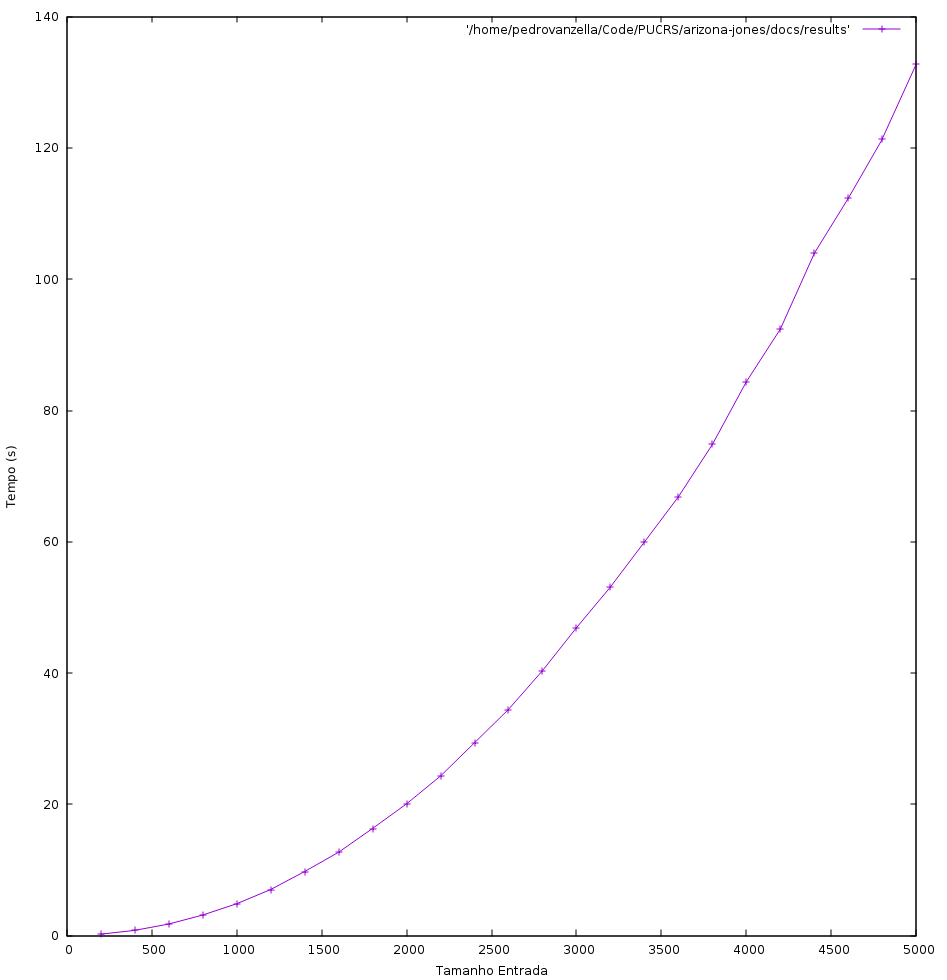
\includegraphics[width=15cm]{results.png}
  \caption{Gráfico de Resultados}
  \label{fig:resultados}
\end{figure}

\end{document}
